% !TEX root = ../main.tex

\section{Data}

\subsection{Elastic Collisions}

\begin{table}[H]
\centering
\caption{Elastic Collision Data}
\vspace{0.5em}
{
    \aboverulesep=0pt
    \belowrulesep=0pt
    \pgfplotstabletypeset[
        col sep=comma,
        string type,
        every head row/.style={
            before row={\toprule 
                       \multicolumn{1}{|c|}{\textbf{Collision}} & 
                       \multicolumn{1}{c|}{\makecell{\textbf{Mass 1} \\ (\si{\kilogram})}} & 
                       \multicolumn{1}{c|}{\makecell{\textbf{Mass 2} \\ (\si{\kilogram})}} & 
                       \multicolumn{2}{c|}{\makecell{\textbf{Initial Vel 1} \\ (\si{\meter\per\second})}} & 
                       \multicolumn{2}{c|}{\makecell{\textbf{Initial Vel 2} \\ (\si{\meter\per\second})}} & 
                       \multicolumn{2}{c|}{\makecell{\textbf{Final Vel 1} \\ (\si{\meter\per\second})}} & 
                       \multicolumn{2}{c|}{\makecell{\textbf{Final Vel 2} \\ (\si{\meter\per\second})}} \\
                       \cmidrule{4-5} \cmidrule{6-7} \cmidrule{8-9} \cmidrule{10-11}
                       & & & \textbf{x} & \textbf{y} & \textbf{x} & \textbf{y} & \textbf{x} & \textbf{y} & \textbf{x} & \textbf{y} \\
                       \midrule},
            after row={}
        },
        every nth row={1}{before row=},
        every last row/.style={
            after row={\bottomrule}
        },
        columns/Collision/.style={
            column name={},
            column type={|l},
            string type
        },
        columns/Mass_1_kg/.style={
            column name={},
            fixed,
            column type={|c},
            precision=2
        },
        columns/Mass_2_kg/.style={
            column name={},
            fixed,
            column type={|c},
            precision=2
        },
        columns/Init_Vel_1x_ms/.style={
            column name={},
            fixed,
            column type={|c},
            precision=2
        },
        columns/Init_Vel_1y_ms/.style={
            column name={},
            fixed,
            column type={|c},
            precision=2
        },
        columns/Init_Vel_2x_ms/.style={
            column name={},
            fixed,
            column type={|c},
            precision=2
        },
        columns/Init_Vel_2y_ms/.style={
            column name={},
            fixed,
            column type={|c},
            precision=2
        },
        columns/Final_Vel_1x_ms/.style={
            column name={},
            fixed,
            column type={|c},
            precision=2
        },
        columns/Final_Vel_1y_ms/.style={
            column name={},
            fixed,
            column type={|c},
            precision=2
        },
        columns/Final_Vel_2x_ms/.style={
            column name={},
            fixed,
            column type={|c},
            precision=2
        },
        columns/Final_Vel_2y_ms/.style={
            column name={},
            fixed,
            column type={|c|},
            precision=2
        }
    ]{data/elastic-collisions.csv}
}
\end{table}

\subsection{Inelastic Collisions}

\begin{table}[H]
\centering
\caption{Inelastic Collision Data}
\vspace{0.5em}
{
    \aboverulesep=0pt
    \belowrulesep=0pt
    \pgfplotstabletypeset[
        col sep=comma,
        string type,
        every head row/.style={
            before row={\toprule 
                       \multicolumn{1}{|c|}{\textbf{Collision}} & 
                       \multicolumn{1}{c|}{\makecell{\textbf{Mass 1} \\ (\si{\kilogram})}} & 
                       \multicolumn{1}{c|}{\makecell{\textbf{Mass 2} \\ (\si{\kilogram})}} & 
                       \multicolumn{2}{c|}{\makecell{\textbf{Initial Vel 1} \\ (\si{\meter\per\second})}} & 
                       \multicolumn{2}{c|}{\makecell{\textbf{Initial Vel 2} \\ (\si{\meter\per\second})}} & 
                       \multicolumn{2}{c|}{\makecell{\textbf{Final Vel 1} \\ (\si{\meter\per\second})}} & 
                       \multicolumn{2}{c|}{\makecell{\textbf{Final Vel 2} \\ (\si{\meter\per\second})}} \\
                       \cmidrule{4-5} \cmidrule{6-7} \cmidrule{8-9} \cmidrule{10-11}
                       & & & \textbf{x} & \textbf{y} & \textbf{x} & \textbf{y} & \textbf{x} & \textbf{y} & \textbf{x} & \textbf{y} \\
                       \midrule},
            after row={}
        },
        every nth row={1}{before row=},
        every last row/.style={
            after row={\bottomrule}
        },
        columns/Collision/.style={
            column name={},
            column type={|l},
            string type
        },
        columns/Mass_1_kg/.style={
            column name={},
            fixed,
            column type={|c},
            precision=2
        },
        columns/Mass_2_kg/.style={
            column name={},
            fixed,
            column type={|c},
            precision=2
        },
        columns/Init_Vel_1x_ms/.style={
            column name={},
            fixed,
            column type={|c},
            precision=2
        },
        columns/Init_Vel_1y_ms/.style={
            column name={},
            fixed,
            column type={|c},
            precision=2
        },
        columns/Init_Vel_2x_ms/.style={
            column name={},
            fixed,
            column type={|c},
            precision=2
        },
        columns/Init_Vel_2y_ms/.style={
            column name={},
            fixed,
            column type={|c},
            precision=2
        },
        columns/Final_Vel_1x_ms/.style={
            column name={},
            fixed,
            column type={|c},
            precision=2
        },
        columns/Final_Vel_1y_ms/.style={
            column name={},
            fixed,
            column type={|c},
            precision=2
        },
        columns/Final_Vel_2x_ms/.style={
            column name={},
            fixed,
            column type={|c},
            precision=2
        },
        columns/Final_Vel_2y_ms/.style={
            column name={},
            fixed,
            column type={|c|},
            precision=2
        }
    ]{data/inelastic-collisions.csv}
}
\end{table}

\subsection{Images}

\begin{figure}[H]
\centering
% Row 1: Elastic Collision 1 (Initial, Final) + Elastic Collision 2 (Initial)
\begin{subfigure}{0.3\textwidth}
    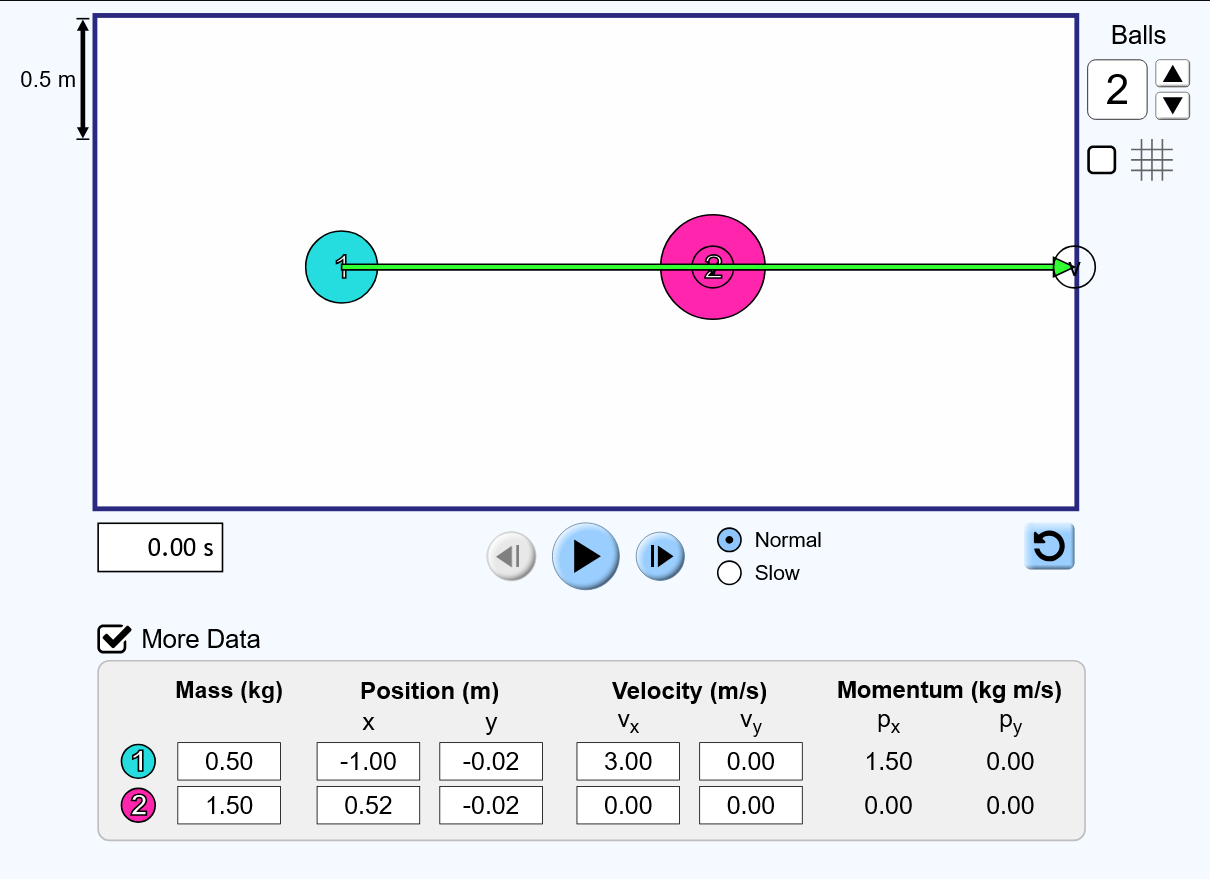
\includegraphics[width=\textwidth]{images/elastic1_initial.png}
    \caption{Elastic 1 - Initial}
    \label{fig:elastic1_initial}
\end{subfigure}
\hfill
\begin{subfigure}{0.3\textwidth}
    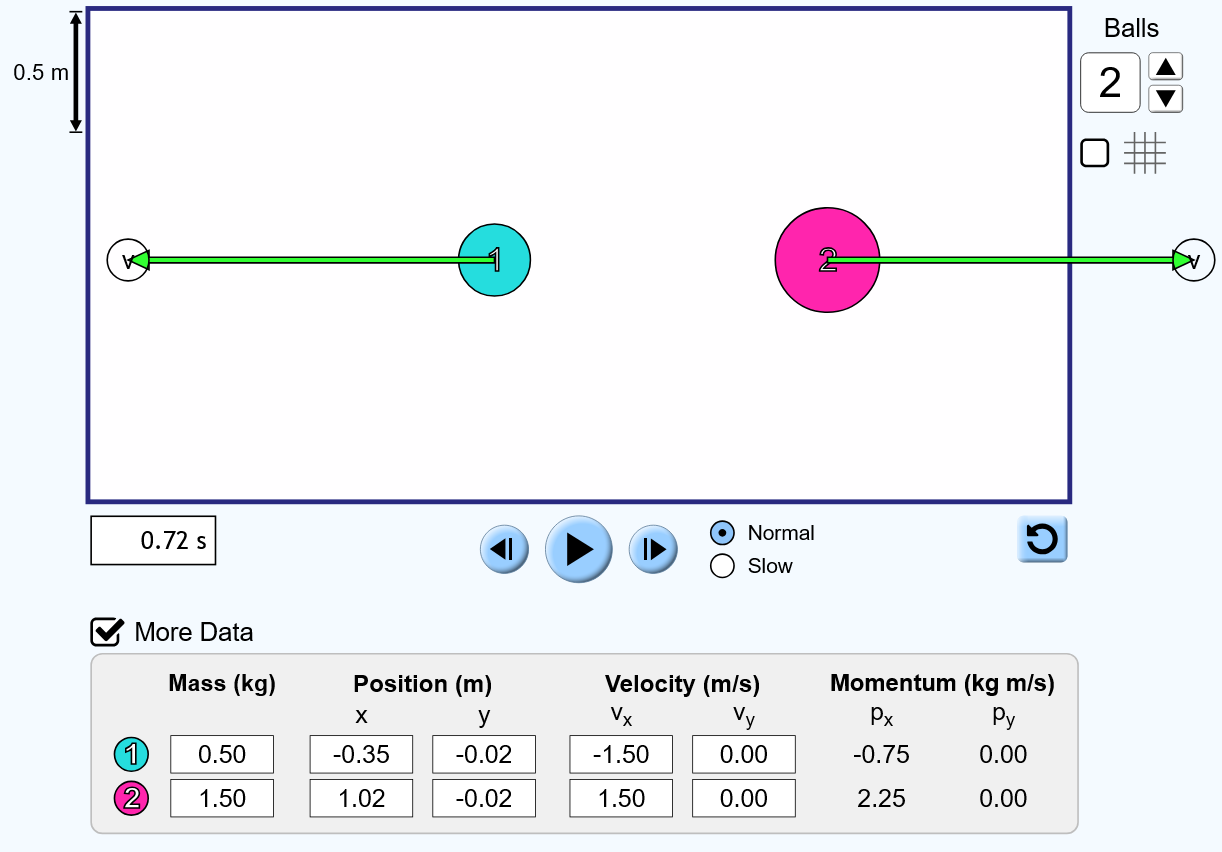
\includegraphics[width=\textwidth]{images/elastic1_final.png}
    \caption{Elastic 1 - Final}
    \label{fig:elastic1_final}
\end{subfigure}
\hfill
\begin{subfigure}{0.3\textwidth}
    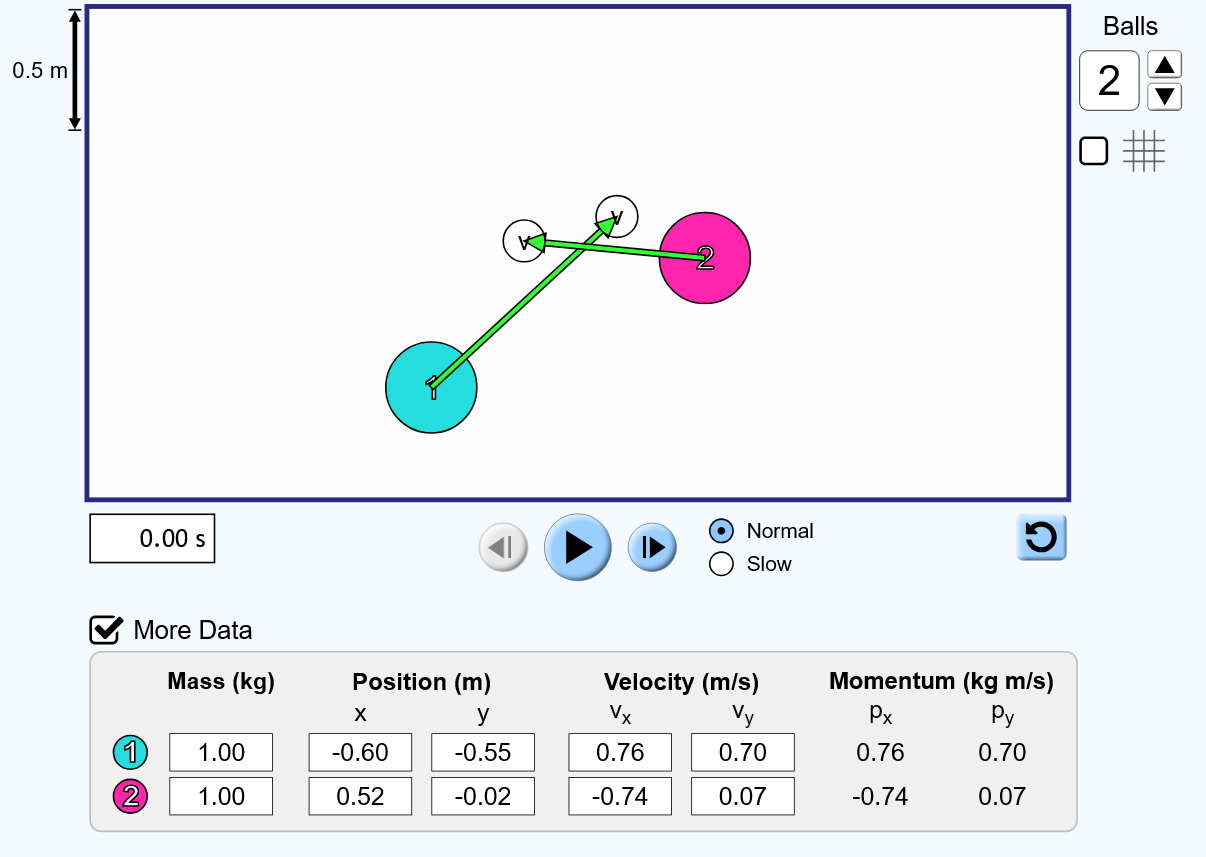
\includegraphics[width=\textwidth]{images/elastic2_initial.png}
    \caption{Elastic 2 - Initial}
    \label{fig:elastic2_initial}
\end{subfigure}

\vspace{0.5em}

% Row 2: Elastic Collision 2 (Final) + Elastic Collision 3 (Initial, Final)
\begin{subfigure}{0.3\textwidth}
    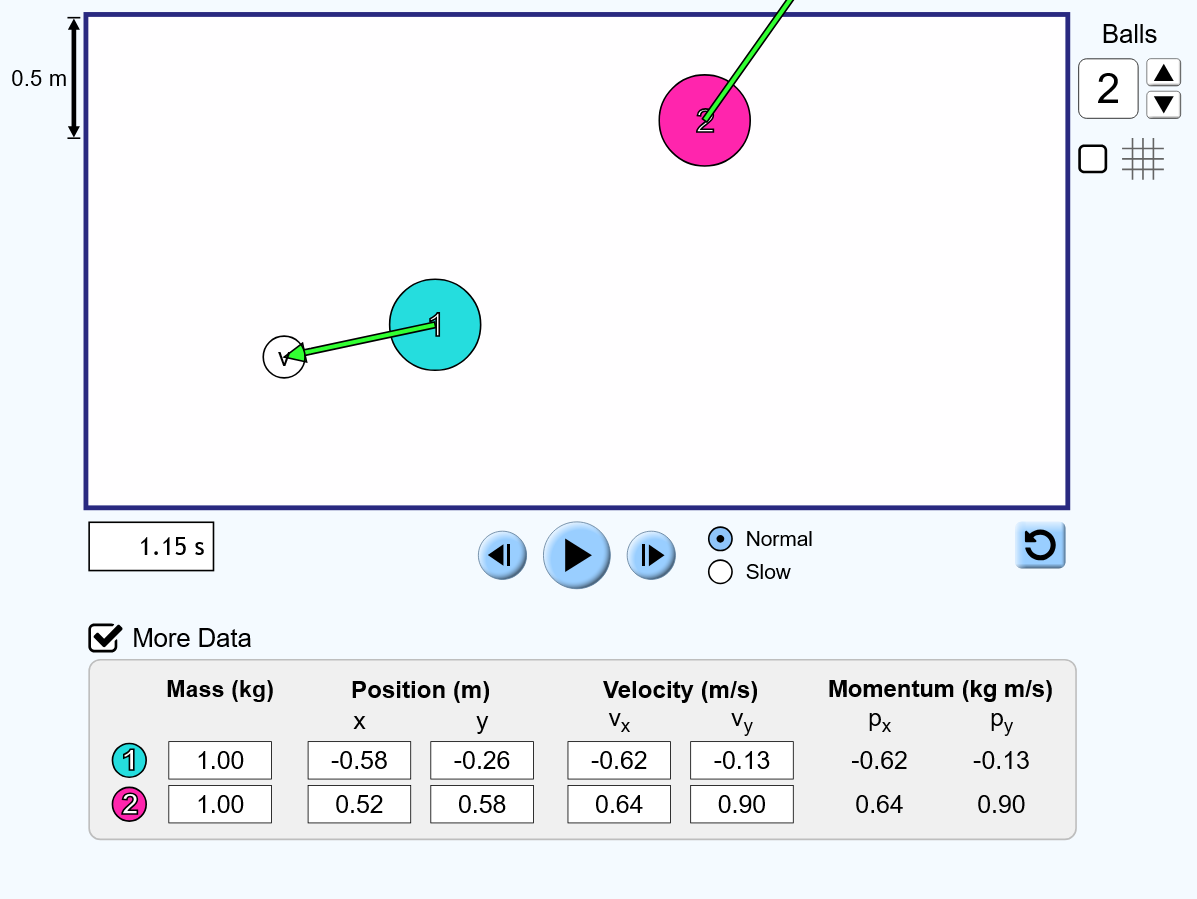
\includegraphics[width=\textwidth]{images/elastic2_final.png}
    \caption{Elastic 2 - Final}
    \label{fig:elastic2_final}
\end{subfigure}
\hfill
\begin{subfigure}{0.3\textwidth}
    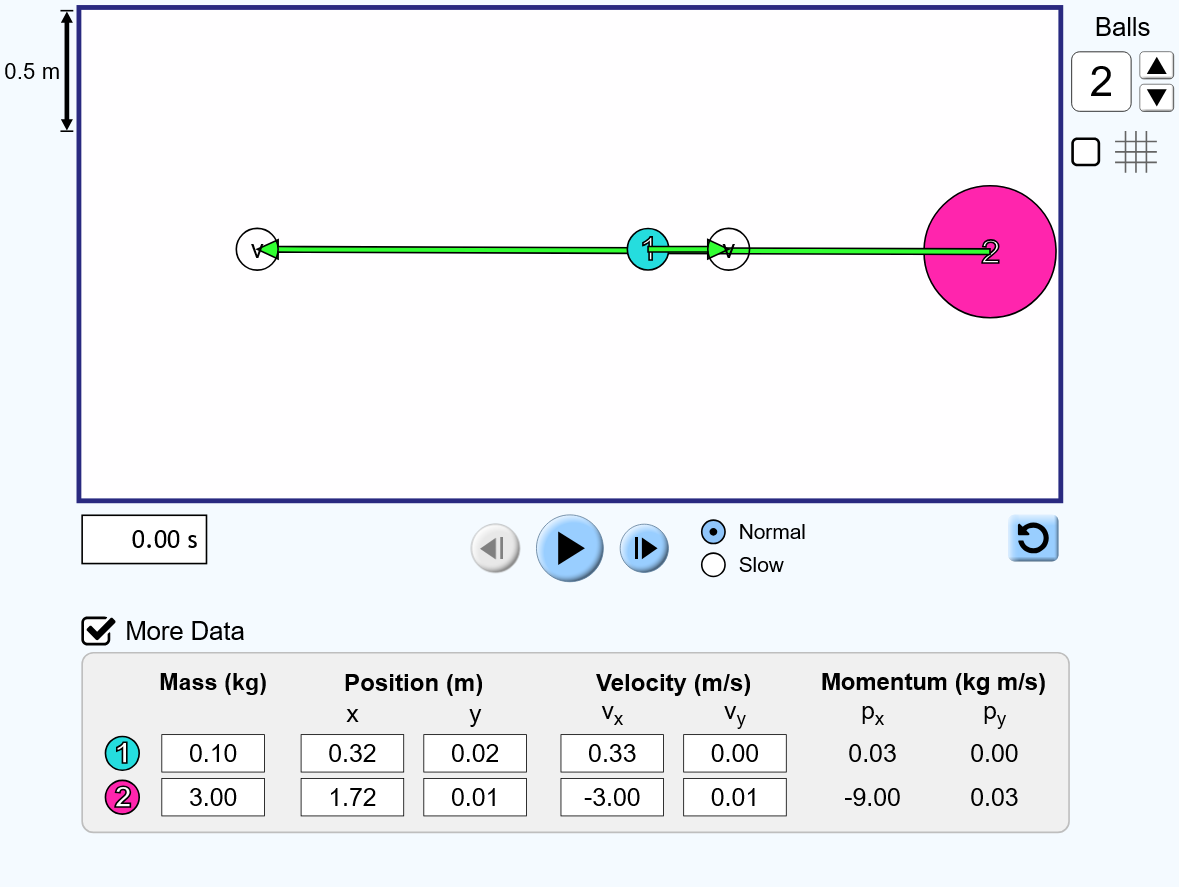
\includegraphics[width=\textwidth]{images/elastic3_initial.png}
    \caption{Elastic 3 - Initial}
    \label{fig:elastic3_initial}
\end{subfigure}
\hfill
\begin{subfigure}{0.3\textwidth}
    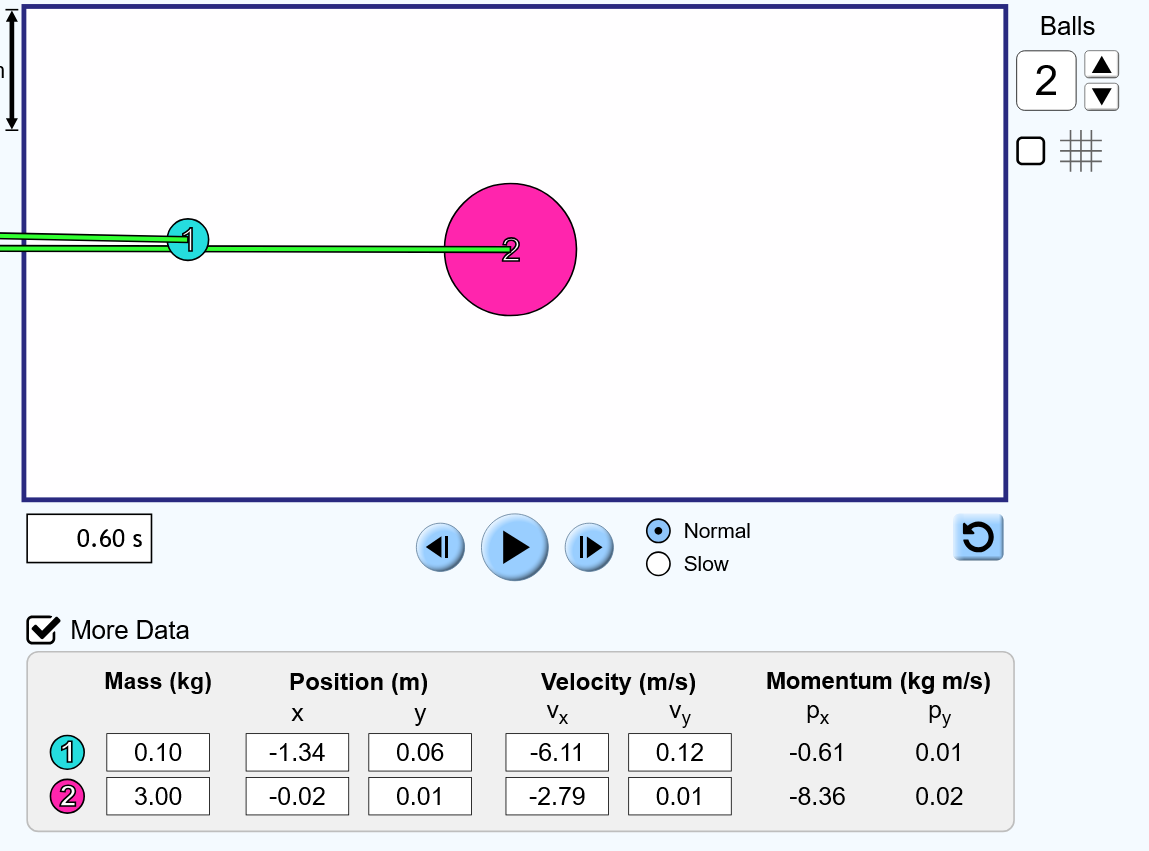
\includegraphics[width=\textwidth]{images/elastic3_final.png}
    \caption{Elastic 3 - Final}
    \label{fig:elastic3_final}
\end{subfigure}

\vspace{0.5em}

% Row 3: Inelastic Collision 1 (Initial, Final) + Inelastic Collision 2 (Initial)
\begin{subfigure}{0.3\textwidth}
    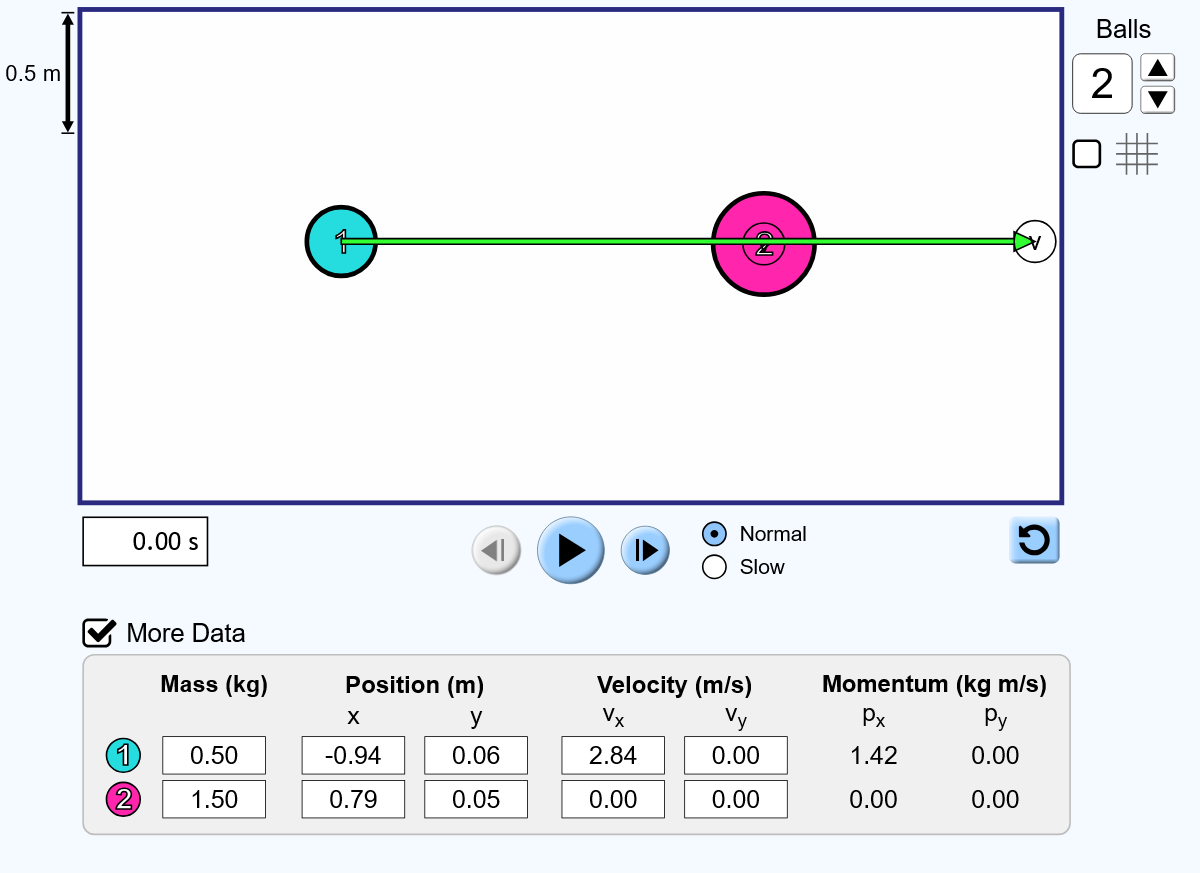
\includegraphics[width=\textwidth]{images/inelastic1_initial.png}
    \caption{Inelastic 1 - Initial}
    \label{fig:inelastic1_initial}
\end{subfigure}
\hfill
\begin{subfigure}{0.3\textwidth}
    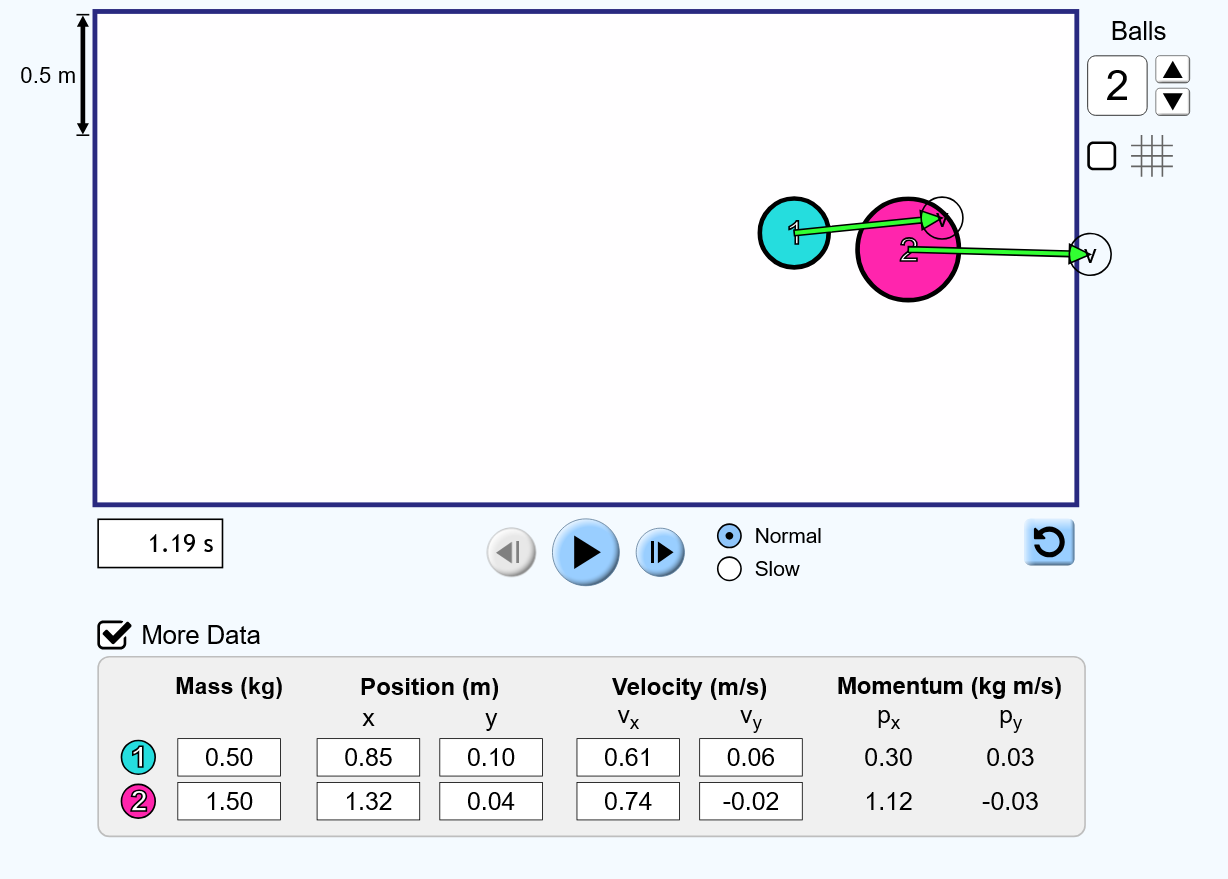
\includegraphics[width=\textwidth]{images/inelastic1_final.png}
    \caption{Inelastic 1 - Final}
    \label{fig:inelastic1_final}
\end{subfigure}
\hfill
\begin{subfigure}{0.3\textwidth}
    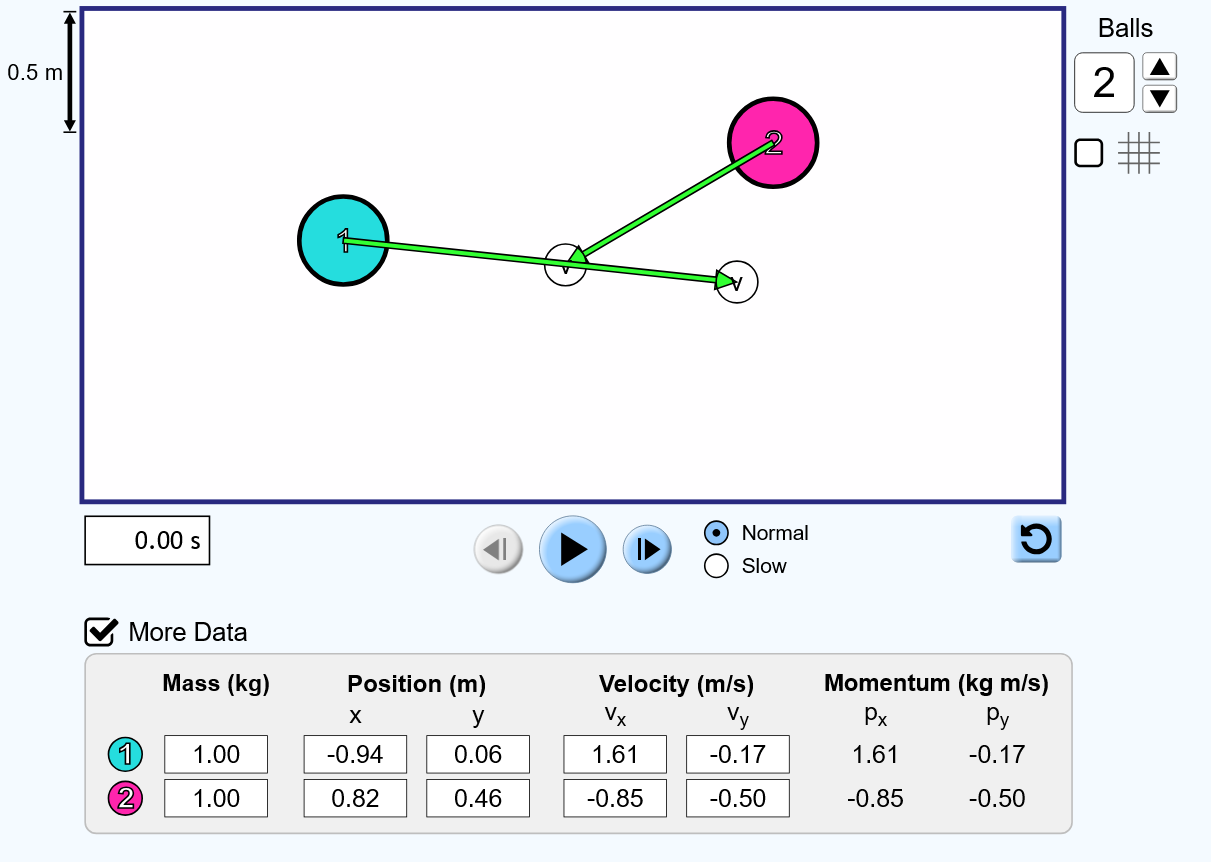
\includegraphics[width=\textwidth]{images/inelastic2_initial.png}
    \caption{Inelastic 2 - Initial}
    \label{fig:inelastic2_initial}
\end{subfigure}

\vspace{0.5em}

% Row 4: Inelastic Collision 2 (Final) + Inelastic Collision 3 (Initial, Final)
\begin{subfigure}{0.3\textwidth}
    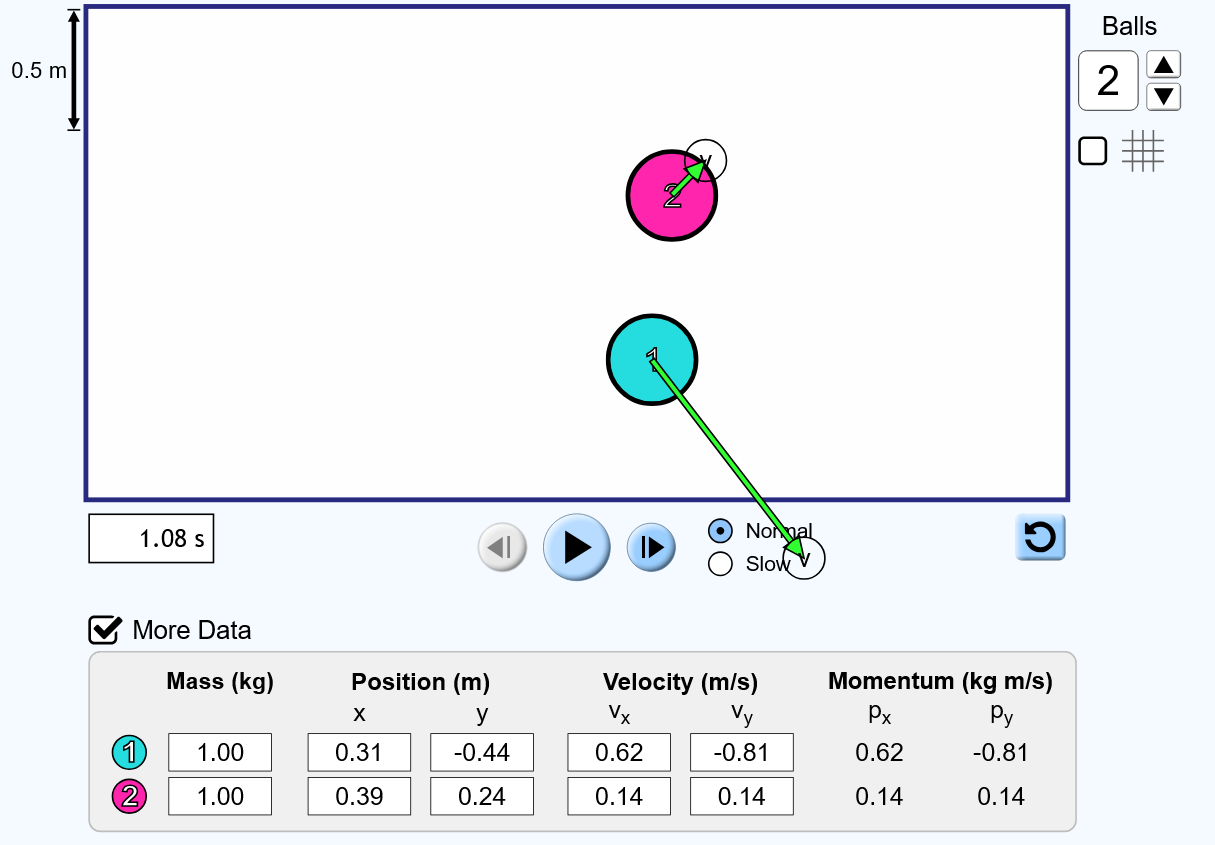
\includegraphics[width=\textwidth]{images/inelastic2_final.png}
    \caption{Inelastic 2 - Final}
    \label{fig:inelastic2_final}
\end{subfigure}
\hfill
\begin{subfigure}{0.3\textwidth}
    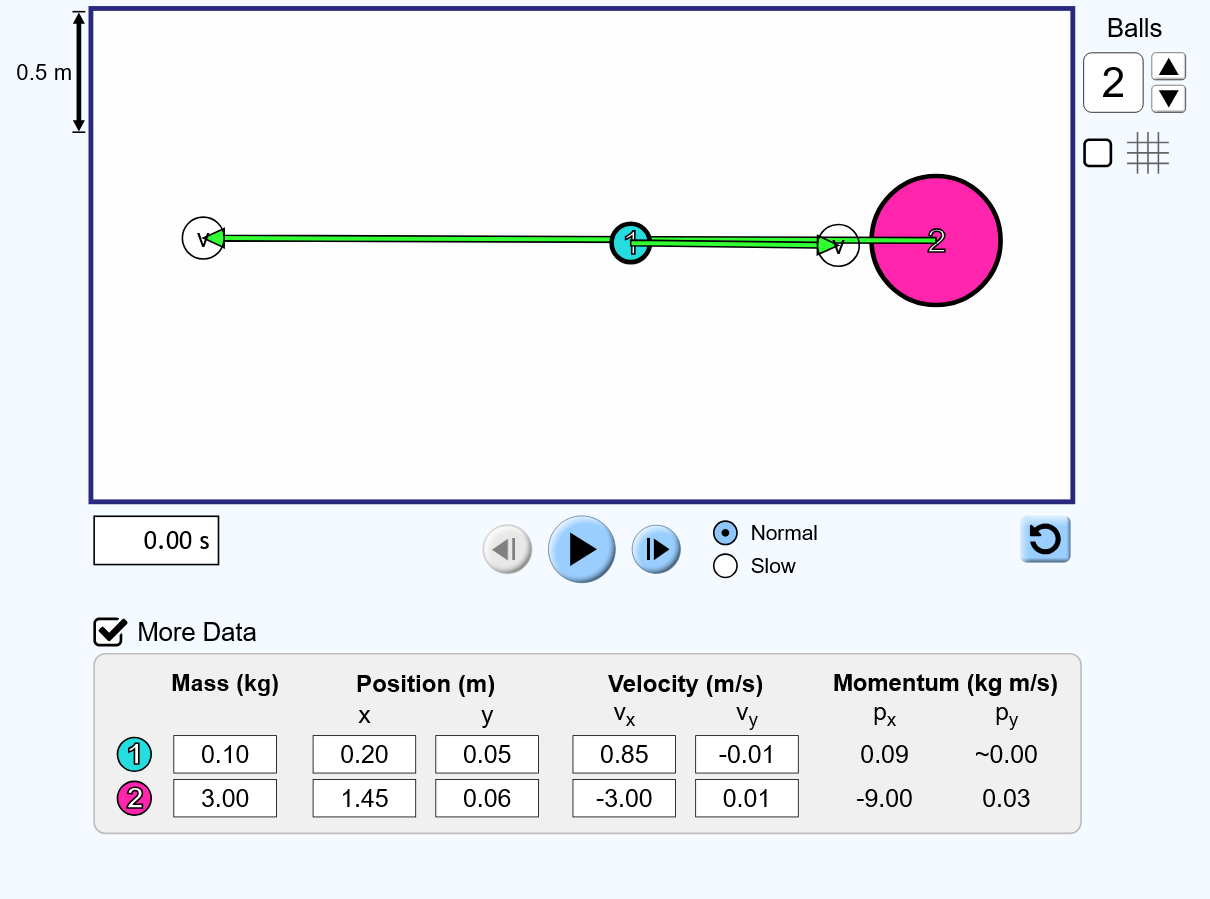
\includegraphics[width=\textwidth]{images/inelastic3_initial.png}
    \caption{Inelastic 3 - Initial}
    \label{fig:inelastic3_initial}
\end{subfigure}
\hfill
\begin{subfigure}{0.3\textwidth}
    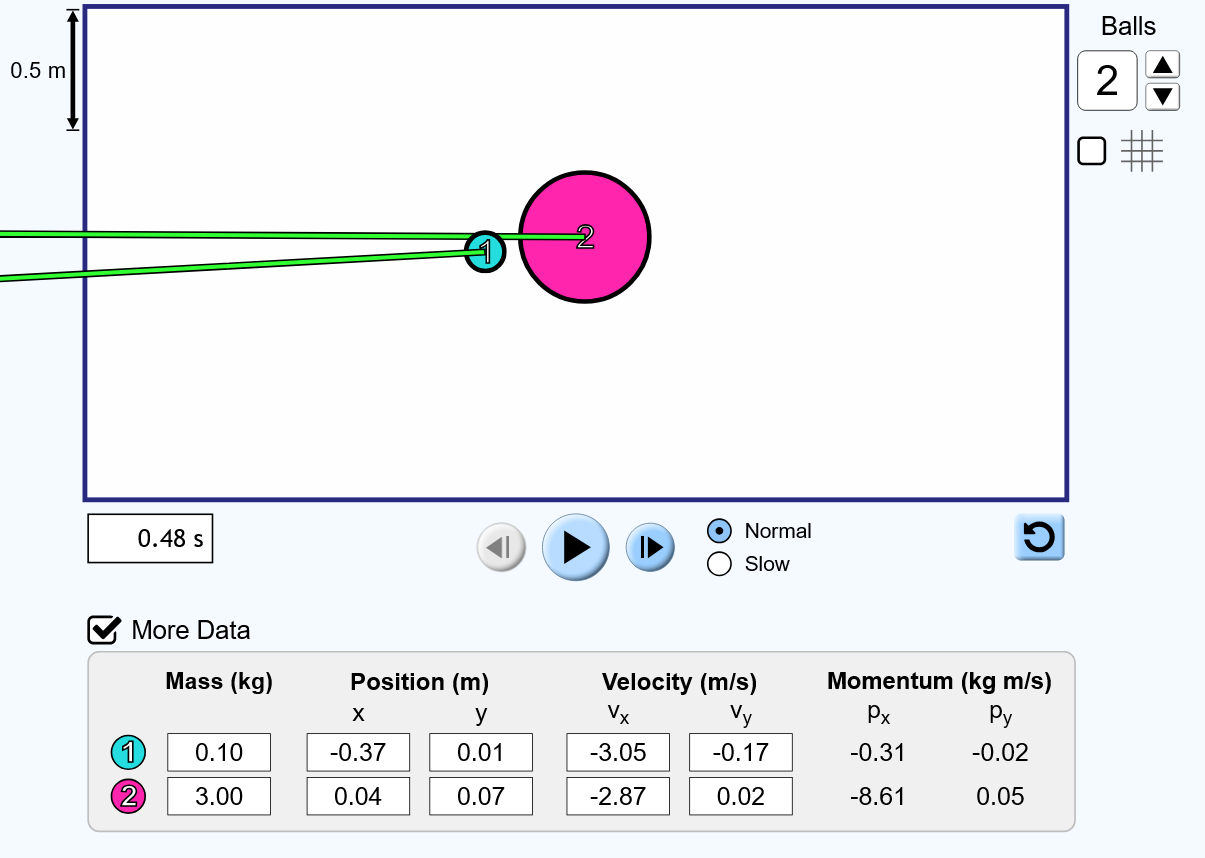
\includegraphics[width=\textwidth]{images/inelastic3_final.png}
    \caption{Inelastic 3 - Final}
    \label{fig:inelastic3_final}
\end{subfigure}

\caption{Collision Images}
\label{fig:collision_images}
\end{figure}